\documentclass[tikz, border=15pt]{standalone}
\usepackage{helvet}
\renewcommand{\familydefault}{\sfdefault}
\usepackage{amsmath}
\usepackage{tikz}
\usetikzlibrary{positioning, arrows.meta, calc, shapes.geometric, decorations.pathreplacing}

\definecolor{emeraldpine}{HTML}{1A4D3E}
\definecolor{harvardcrimson}{HTML}{A51C30}
\definecolor{ethdarkblue}{HTML}{1F407A}
\definecolor{ethpetrol}{HTML}{007A87}
\definecolor{ethbronze}{HTML}{B87333}
\definecolor{ink}{HTML}{1A202C}
\definecolor{cardbg}{HTML}{F8FAFC}
\definecolor{softink}{HTML}{4A5568}

\begin{document}
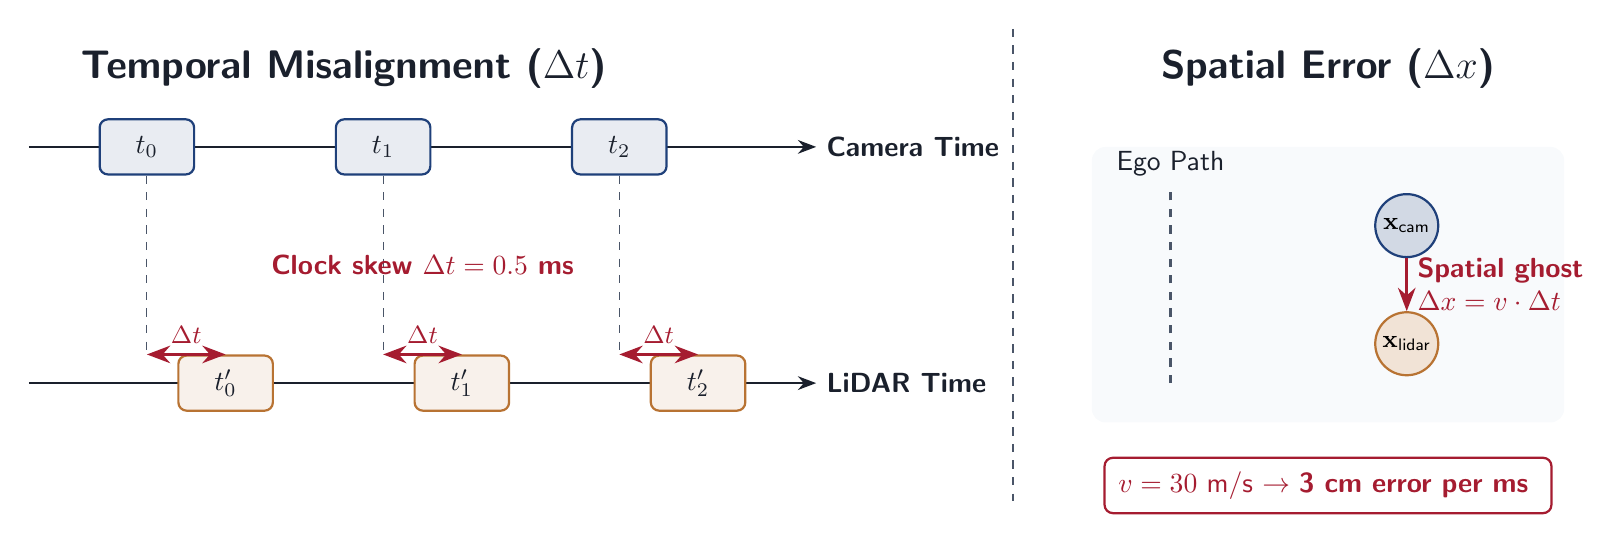
\begin{tikzpicture}[>=Stealth,
    node distance=1cm,
    cam/.style={rectangle, rounded corners=3pt, draw=ethdarkblue, fill=ethdarkblue!10, thick, minimum width=1.2cm, minimum height=0.7cm, text=ink},
    lidar/.style={rectangle, rounded corners=3pt, draw=ethbronze, fill=ethbronze!10, thick, minimum width=1.2cm, minimum height=0.7cm, text=ink},
    font=\sffamily]

    % Left Side: Timeline
    \node[text=ink, font=\sffamily\Large\bfseries] (title_left) at (3, 2.5) {Temporal Misalignment ($\Delta t$)};
    
    % Timelines
    \draw[->, thick, ink] (-1, 1.5) -- (9.0, 1.5) node[right] {\textbf{Camera Time}};
    \draw[->, thick, ink] (-1, -1.5) -- (9.0, -1.5) node[right] {\textbf{LiDAR Time}};
    
    % Camera events
    \node[cam] (c0) at (0.5, 1.5) {$t_0$};
    \node[cam] (c1) at (3.5, 1.5) {$t_1$};
    \node[cam] (c2) at (6.5, 1.5) {$t_2$};
    
    % LiDAR events (skewed by dt)
    \node[lidar] (l0) at (1.5, -1.5) {$t'_0$};
    \node[lidar] (l1) at (4.5, -1.5) {$t'_1$};
    \node[lidar] (l2) at (7.5, -1.5) {$t'_2$};
    
    % Draw projection lines and Delta t arrows
    \foreach \c/\l in {c0/l0, c1/l1, c2/l2} {
        \draw[dashed, softink] (\c.south) -- (\c.south |- \l.north);
        \draw[<->, harvardcrimson, very thick] (\c.south |- \l.north) -- (\l.north) node[midway, above, font=\sffamily\small] {$\Delta t$};
    }
    
    \node[harvardcrimson, font=\sffamily\bfseries] at (4.0, 0) {Clock skew $\Delta t = 0.5$ ms};

    % Divider
    \draw[dashed, softink, thick] (11.5, 3) -- (11.5, -3);

    % Right Side: Spatial consequence
    \begin{scope}[shift={(15.5, 0)}]
    \node[text=ink, font=\sffamily\Large\bfseries] (title_right) at (0, 2.5) {Spatial Error ($\Delta x$)};
    
    % Bird's eye view box
    \draw[fill=cardbg, draw=none, rounded corners=5pt] (-3, -2) rectangle (3, 1.5);
    \draw[dashed, thick, softink] (-2, -1.5) -- (-2, 1) node[above, text=ink] {Ego Path};
    
    \node[circle, draw=ethdarkblue, fill=ethdarkblue!20, minimum size=0.8cm, inner sep=0, thick, font=\sffamily\small] (x_cam) at (1, 0.5) {$\mathbf{x}_{\text{cam}}$};
    \node[circle, draw=ethbronze, fill=ethbronze!20, minimum size=0.8cm, inner sep=0, thick, font=\sffamily\small] (x_lidar) at (1, -1.0) {$\mathbf{x}_{\text{lidar}}$};
    
    \draw[->, harvardcrimson, very thick] (x_cam.south) -- (x_lidar.north) node[midway, right, align=left, font=\sffamily] {
        \textbf{Spatial ghost}\\
        $\Delta x = v \cdot \Delta t$
    };
    
    \node[draw=harvardcrimson, fill=white, thick, rounded corners=3pt, align=center, text=harvardcrimson, inner sep=5pt] at (0, -2.8) {
        $v = 30$ m/s $\rightarrow$ \textbf{3 cm error per ms}
    };
    
    \end{scope}

\end{tikzpicture}
\end{document}
